\section{Module stacking}

\textbf{Module 1 code below, declare the my\_add function}
\newline
\text{Using \textit{EXPORT\_SYMBOL} to export symbol}
\begin{lstlisting}[style=CStyle]
    #include <linux/kernel.h>
    #include <linux/module.h>
    
    MODULE_LICENSE("GPL");
    
    int my_add(int a, int b) {
        return a + b;
    }
    EXPORT_SYMBOL(my_add);
    
    static int test_init(void) {
        printk(KERN_INFO"%s: In init by module1\n", __func__);
    
        return 0;
    }
    
    static void test_exit(void) {
        printk(KERN_INFO"%s: In exit by module1: \n", __func__);
    }
    
    module_init(test_init);
    module_exit(test_exit);
    
    MODULE_AUTHOR("Danny Deng");
    MODULE_DESCRIPTION("Argument parsing example");    
\end{lstlisting}

\textbf{Module 2 code below, call the my\_add function}
\begin{lstlisting}[style=CStyle]
    #include <linux/kernel.h>
    #include <linux/module.h>

    MODULE_LICENSE("GPL");

    /* Define in module1.c and already EXPORT_SYMBOL */
    extern int my_add(int a, int b);

    static int test_init(void) {
        printk(KERN_INFO"%s: In init by module2\n", __func__);
        printk(KERN_INFO"my_add(1, 2): %d\n", my_add(1, 2));
        return 0;
    }

    static void test_exit(void) {
        printk(KERN_INFO"%s: In exit by module2: \n", __func__);
    }

    module_init(test_init);
    module_exit(test_exit);

    MODULE_AUTHOR("Danny Deng");
    MODULE_DESCRIPTION("Argument parsing example");
\end{lstlisting}




\textbf{Result}
\begin{center}
    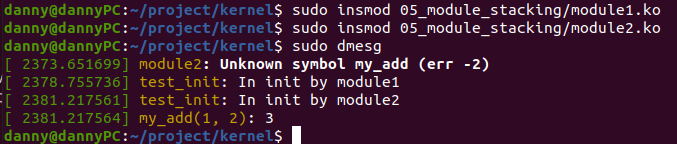
\includegraphics[width=\linewidth]{images/05_module_stacking.png}
\end{center}

